\let\negmedspace\undefined
\let\negthickspace\undefined

\documentclass[journal]{IEEEtran}
\usepackage[a5paper, margin=10mm, onecolumn]{geometry}
\usepackage{tfrupee}

\setlength{\headheight}{1cm}
\setlength{\headsep}{0mm}

\usepackage{gvv-book}
\usepackage{gvv}
\usepackage{cite}
\usepackage{amsmath,amssymb,amsfonts,amsthm}
\usepackage{algorithmic}
\usepackage{graphicx}
\usepackage{textcomp}
\usepackage{xcolor}
\usepackage{txfonts}
\usepackage{listings}
\usepackage{enumitem}
\usepackage{mathtools}
\usepackage{gensymb}
\usepackage{comment}
\usepackage[breaklinks=true]{hyperref}
\usepackage{tkz-euclide} 
\usepackage{listings}
\def\inputGnumericTable{}                                 
\usepackage[latin1]{inputenc}                                
\usepackage{color}                                            
\usepackage{array}                                            
\usepackage{longtable}                                       
\usepackage{calc}                                             
\usepackage{multirow}                                         
\usepackage{hhline}                                           
\usepackage{ifthen}                                           
\usepackage{lscape}
\begin{document}

\bibliographystyle{IEEEtran}
\vspace{3cm}

\title{5.8.8}
\author{EE25BTECH11010 - Arsh Dhoke}
{\let\newpage\relax\maketitle}

\renewcommand{\thefigure}{\theenumi}
\renewcommand{\thetable}{\theenumi}
\setlength{\intextsep}{10pt}
\numberwithin{equation}{enumi}
\numberwithin{figure}{enumi}
\renewcommand{\thetable}{\theenumi}

\parindent 0px
\textbf{Question}:\\
Places A and B are 100km apart on a highway. One car starts from A and another from B at the same time. If the cars travel in the same direction at different speeds, they meet in 5hrs. If they travel towards each other, they meet in 1hr. What are the speeds of the two cars?

\solution \\
Let the speeds be $v_1$ and $v_2$ (in km/h). From the two cases,
\begin{align}
\label{eq:sys1} v_1 + v_2 &= 100, \\
\label{eq:sys2} v_1 - v_2 &= 20.
\end{align}

These can be written in vector form as
\begin{align}
\myvec{1 & 1} \myvec{v_1 \\ v_2} &= 100, \\
\myvec{1 & -1} \myvec{v_1 \\ v_2} &= 20.
\end{align}

Let 
\begin{align}
\vec{r_1} = \myvec{1 & 1}, \quad \vec{r_2} = \myvec{1 & -1}.
\end{align}
Then \(\vec{r_1}\cdot\vec{r_2}=0\), so the rows are orthogonal.

Let
\begin{align}
\myvec{v_1 \\ v_2} = c_1\,\vec{r_1}^{T} + c_2\,\vec{r_2}^{T}.
\end{align}

Taking dot products of both sides with \(\vec{r_1}\) and \(\vec{r_2}\):
\begin{align}
\vec{r_1}\cdot\myvec{v_1 \\ v_2} &= c_1\,\vec{r_1}\cdot\vec{r_1} = 100, \\
\vec{r_2}\cdot\myvec{v_1 \\ v_2} &= c_2\,\vec{r_2}\cdot\vec{r_2} = 20.
\end{align}

Since \(\|\vec{r_1}\|^2 = \|\vec{r_2}\|^2 = 2\), we have
\begin{align}
c_1 = \frac{100}{2} = 50, \quad c_2 = \frac{20}{2} = 10.
\end{align}

Thus,
\begin{align}
\myvec{v_1 \\ v_2} &= 50\,\vec{r_1}^{T} + 10\,\vec{r_2}^{T} \\
&= 50\myvec{1 \\ 1} + 10\myvec{1 \\ -1} \\
&= \myvec{60 \\ 40}.
\end{align}

\begin{align}
\therefore \quad v_1 = 60~\text{km/h}, \quad v_2 = 40~\text{km/h}.
\end{align}

\begin{figure}[ht!]
\centering
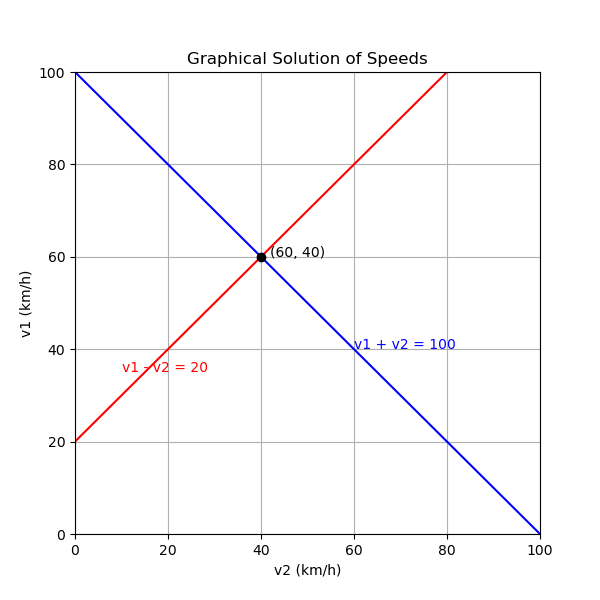
\includegraphics[height=0.6\textheight, keepaspectratio]{figs/speed.png}
\captionof{figure}{Graph}
\end{figure}

\end{document}